% !TeX root = ../main.tex
\chapter{Project 04: Target tracking under sparse sensor attacks}

\section{Objectives}
The aim of this project is to track the position of a device using RSS fingerprinting setting. In this project, we are given the dictionary $D$, and it is requested to track the position of the device having a given noisy and attack corrupted measurements.

\section{Setting of the problem}
In this task, the room is gridded into 36 cells and 20 sensors are used in the training phase. In addition, it is assumed that during the training step has done in an offline manner, and therefore, the dictionary $D$ is assumed to be attack free. During the ``application'' phase, which it is required to track the position a device, 4 sensors are under the attack, and the task is to track the position of a target, or targets in this room given the dynamical evolution of the system, and also find which sensors are under attack. The model has the following dynamics:

\begin{equation}
\begin{cases}
x(k+1) = A\,x(k) \\
y(k) = D\,x(k) + \tilde{a} + \eta
\end{cases}
\end{equation}

where the measurement vector $y(k)$ is corrupted by a constant attack vector $\tilde{a}$ and noise $\eta$.

The same as the previous project, the problem to be solved is sparse. The same as \textit{task 2}, a full weighted Lasso needs to be considered, since the position of a target or some targets in a room are assumed to be sparse:

\begin{equation}
\min_{x \in \mathbb{R}^{n}, a \in \mathbb{R}^{q}} \left\| G \begin{pmatrix} x \\ a \end{pmatrix} - y \right\|_2^2 + \lambda_1 \| x \|_1 + \lambda_2 \| a \|_1
\end{equation}
where,
\[
G = (D, I)
\]

Here, in order not to face numerical problems, G should be normalized, this is done using \texttt{normalize( )} command in MATLAB. In this way, we make sure that $G$ and $I$ are of the same scale.

\section{Implementation of the algorithm}
\subsection{Luenberg Observer}
Since the attacks is assumed to be constant, when shaping the observability matrix, at least 2 columns are going to be linearly dependent, and hence, some states are going to be unobservable. Therefore, a Luenberg observer cannot be adopted. However, Sparse observers still can be used in order to accomplish the task.

\subsection{SSO for tracking}
SSO can be adopted in order to solve the problem; however, the terms regarding the state needs to be sparsified

\textbf{Initialization:} \(\tau > 0\), \(\hat{x}(0) \in \mathbb{R}^{n}\), \(\hat{a}(0) \in \mathbb{R}^{q}\), e.g., \(\hat{x}(0) = 0\), \(\hat{a}(0) = 0\)

\textbf{For} \( k = 0, \dots, T_{\max} \),

\begin{align}
    y(k) &= D_1x(k) + a\\
    \hat{y}(k) &= D_1\hat{x}(k) + \hat{a}\\
    \hat{x}(k+1) &= S_{\nu_1\lambda_1} [A\hat{x}(k) - \nu A D_1^\top (\hat{y}(k) - y(k))] \\
    \hat{a}(k+1) &= S_{\nu_2\lambda_2} [\hat{a}(k) - \nu I_1^\top (\hat{y}(k) - y(k))] \\
    x(k+1) &= A x(k)
\end{align}
where $D_1$ and $I_1$ are normalized $D$ and $I$

The suggested values of hyperparameters used in this algorithm are:
\begin{itemize}
	\item $\lambda_1 = \lambda_2 = 10$
	\item $\nu_1 = \frac{0.99}{\|D_1\|_2^2}$
	\item $\nu_2 = \frac{0.99}{\|I_1\|_2^2}$
\end{itemize} 
To enhance the convergence rate the following values were used for SSO:
\begin{itemize}
	\item $\lambda_1 = \lambda_2 = 10$
	\item $\nu_1 = \frac{2*0.99}{\|D_1\|_2^2}$
	\item $\nu_2 = \frac{2*0.99}{\|I_1\|_2^2}$
\end{itemize} 
To check the perforamance, the performance needs to be cleaned. In the sense that since the value of the state can be either 0 or 1,  a threshold should be considered so that for the values of the states lower than that threshold the state becomes 0 and otherwise, 1. A threshold of 0.1 was considered for this algorithm.
\subsection{D-SSO for tracking}
The taylored D-SSO for tracking is as follows:

\textbf{For} \( k = 0, \dots, T_{\max} \),

\begin{align}
    y(k) &= Cx(k) + a(k) \\
    \hat{y}(k) &= C\hat{x}(k) + \hat{a}(k) \\
    \hat{x}(k+1) &= S_{\nu\lambda}[A\hat{x}(k) - L (\hat{y}(k) - y(k))] \\
    \hat{a}(k+1) &= S_{\nu\lambda} [\hat{a}(k) - \nu (\hat{y}(k) - y(k))] \\
    x(k+1) &= A x(k)
\end{align}

Where $L$ is designed such that, $eig(A - LC) = 0$. In order not to face numerical issues, \texttt{place()} command is used by randomized desirable eigenvalues close enough to zero, with standard deviation of 0.01. The value of hyperparameters used in this algorithm are:
\begin{itemize}
	\item $\lambda = 0.01$
	\item $\nu = 0.05$
\end{itemize} 

The cleaning threshold used for the states is 0.6.

\section{Results}
\subsection{State Support Error}
It is observed that both SSO and DSSO after some iterations can correctly track the position of the target. In terms of performance, SSO correctly tracks the position of the target after 25 iterations with enhanced parameters and after 32 iterations for the suggested hyperparameters. On the otherhand, it took 185 iteration for DSSO to perfectly track the target, which is considerably slower.

\begin{figure}[H]
    \centering
    \subfloat[State support error of SSO using suggested hyperparameters]{
        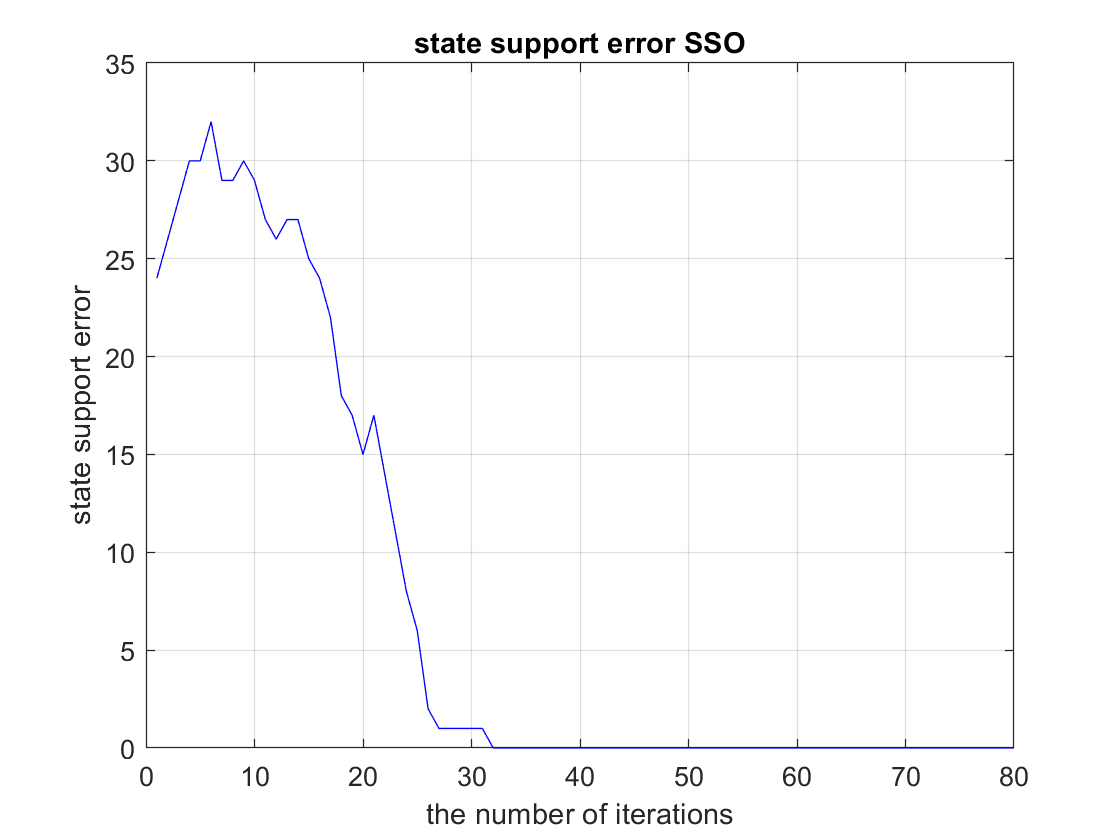
\includegraphics[width=0.45\textwidth]{state_support_error_SSO_suggested.png} % Adjust width as needed
    }
    \hspace{1cm} % Adjust the space between the two figures
    \subfloat[State support error of SSO using enhanced hyperparameters.]{
        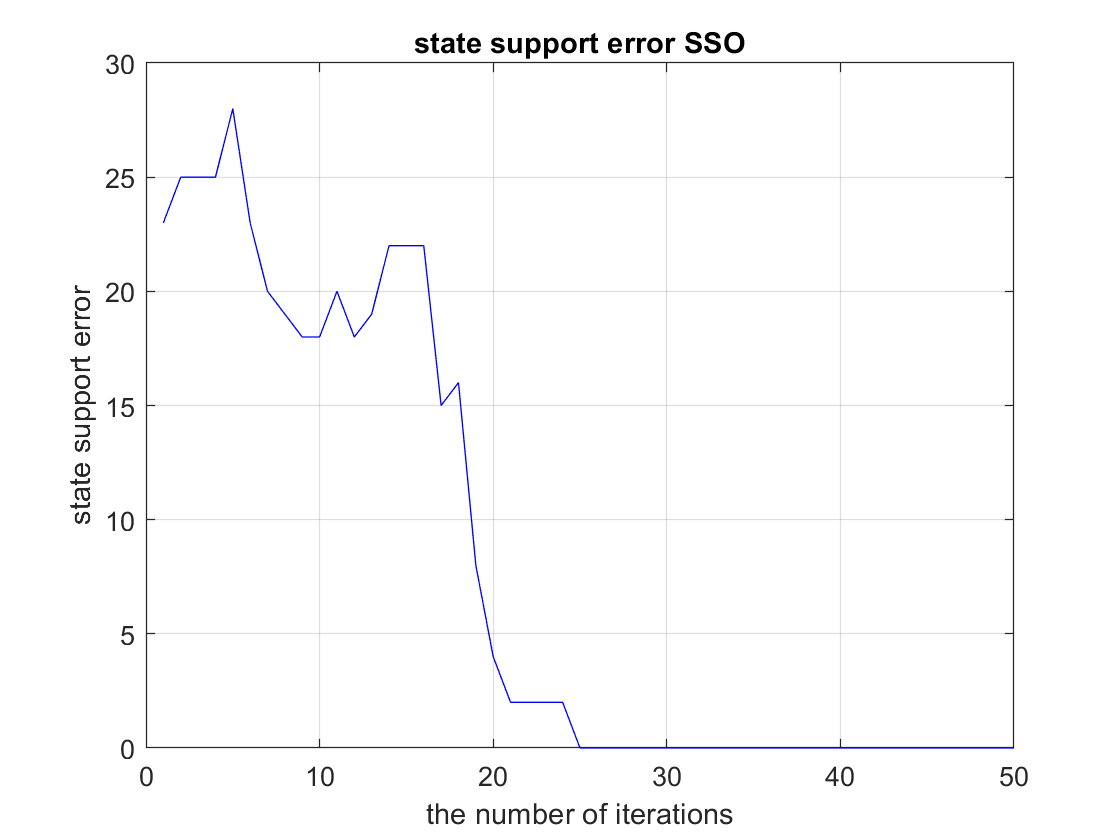
\includegraphics[width=0.45\textwidth]{state_support_error_SSO.png} % Adjust width as needed
    }
    \caption{Comparison of the convergence rate of state support error of SSO using suggested and enhanced hyperparameters for running the algorithm}
\end{figure}

\begin{figure}[H]
    \centering
    \subfloat[tracking performance using suggested hyperparameters]{
        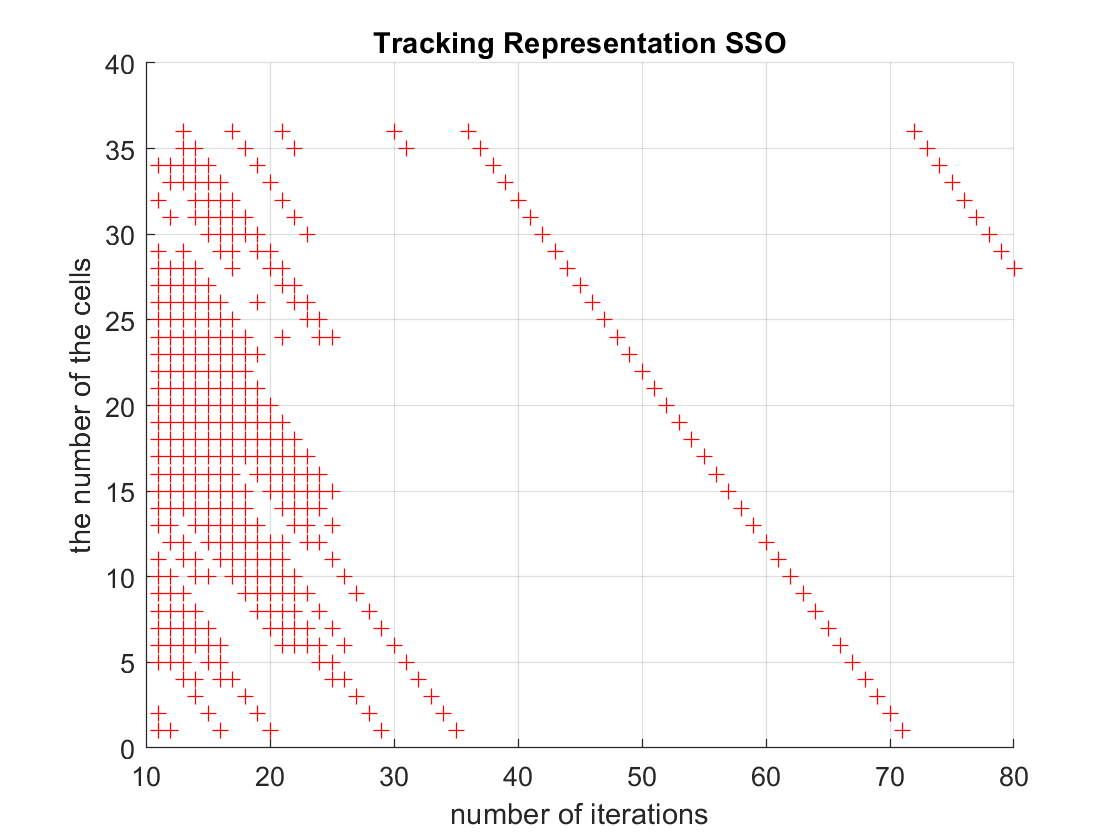
\includegraphics[width=0.45\textwidth]{tracking_SSO_suggested.png} % Adjust width as needed
    }
    \hspace{1cm} % Adjust the space between the two figures
    \subfloat[tracking performance using enhanced hyperparameters.]{
        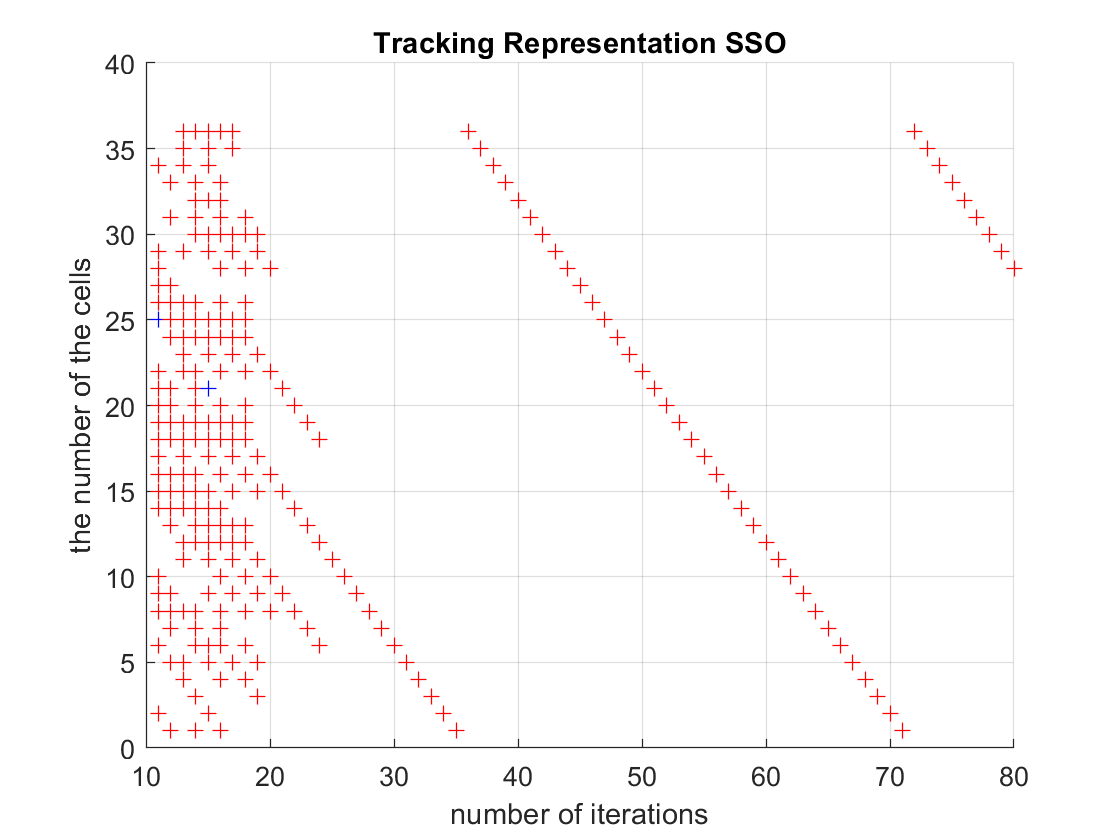
\includegraphics[width=0.45\textwidth]{tracking_SSO.png} % Adjust width as needed
    }
    \caption{Comparison of tracking performance of SSO using suggested and enhanced hyperparameters for running the algorithm}
\end{figure}

As it was also mentioned in the second project, the DSSO, which is the dynamic counterpart of IJAM, does not have a smooth transient, which in turn introduces problem when soft-thresholding is applied. Here, the parameters were turned so that it can solve the problem. However, again a two step approach as it is discussed in the further discussion of the second project can be adopted. Here, a normal approach was adopted and a slower performance from DSSO was observed, which can be since in the following plots.

\begin{figure}[H] % h means "here", can also use t (top), b (bottom), p (page)
    \centering
    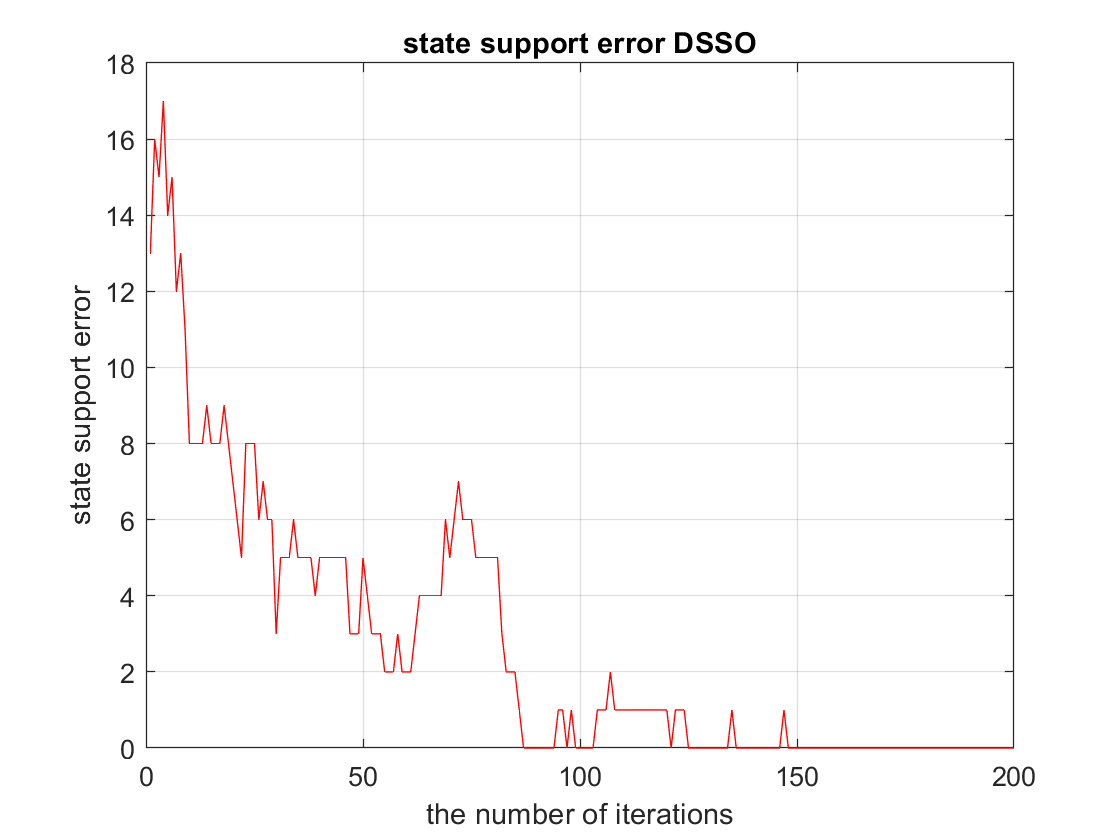
\includegraphics[width=0.75\textwidth]{state_support_error_DSSO.png} % Adjust width as needed
    \caption{State support error of DSSO; it can be seen that it is considerably slower than SSO.}
\end{figure}

\begin{figure}[H] % h means "here", can also use t (top), b (bottom), p (page)
    \centering
    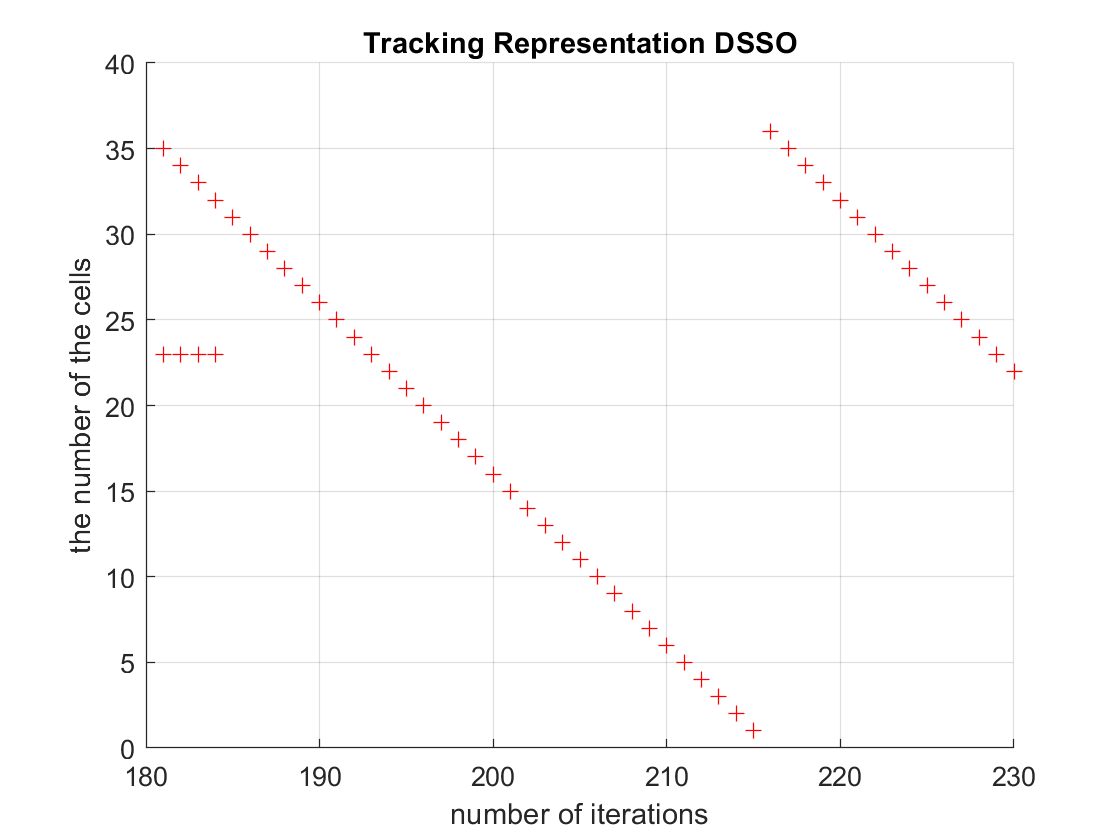
\includegraphics[width=0.75\textwidth]{tracking_DSSO.png} % Adjust width as needed
    \caption{Tracking performance of DSSO}
\end{figure}
\subsection{Attack Support Error:}
Regarding this performance metric, it need to be mentioned that the implemented DSSO is unable to estimate the position of the attacks correcty, and the number of attack support error remain constant on 11. On the other hand, attack support error in the case of SSO convergese to 0 after 20 iterations.
\begin{figure}[H] % h means "here", can also use t (top), b (bottom), p (page)
    \centering
    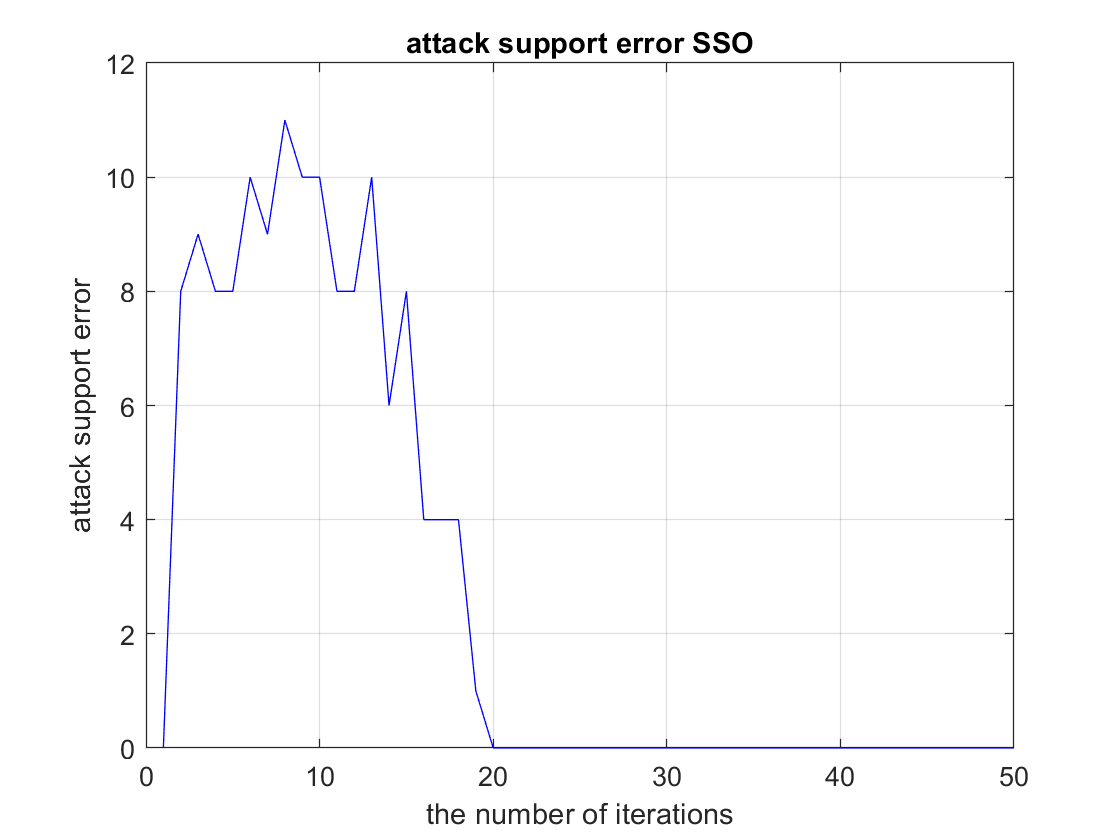
\includegraphics[width=0.75\textwidth]{attack_support_error_SSO.png} % Adjust width as needed
    \caption{Attack support error of SSO}
\end{figure}

\begin{figure}[H] % h means "here", can also use t (top), b (bottom), p (page)
    \centering
    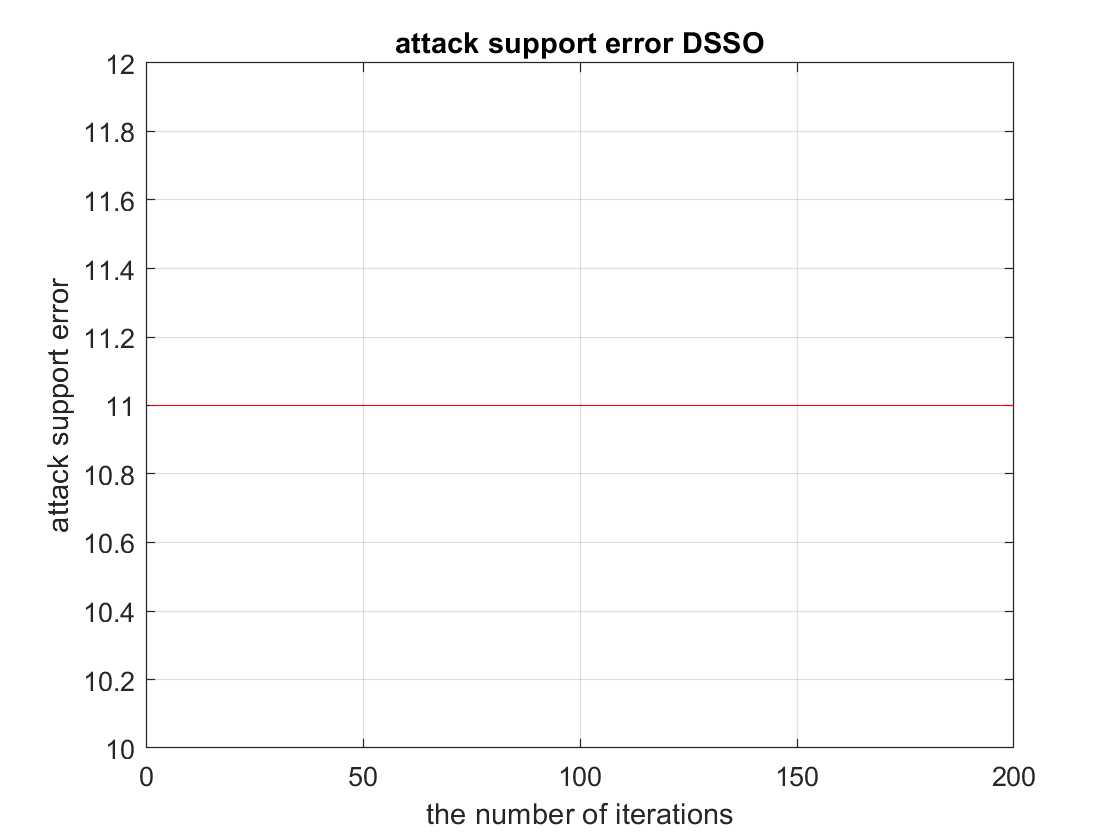
\includegraphics[width=0.75\textwidth]{attack_support_error_DSSO.png} % Adjust width as needed
    \caption{Attack support error of DSSO; the attack support error does not improves over time; since the threshold for cleaning was relatively large, no cleaning threshold was adopted here.}
\end{figure}


\section{Conclusion}
In conclusion, for performing a fingerprint tracking with constant attack, Luenberg observer cannot be used, since the extended observability matrix does not become full rank. Nonetheless, using SSO and DSSO taylored for this problem, which requires introducing soft-thresholding also for the states, tracking was achieved. 

SSO showed a noticably faster performance in tracking compared to DSSO, and unlike DSSO, SSO was able to detect correctly the position of the attacks, DSSO. SSO has a smooth transient and when soft-thresholding is introduced to the problem, it can solve the problem. In the case of DSSO, the introduction of soft-thresholding disrupt the performance of DSSO, owing to the fact that DSSO have an oscillatory transient behavior.

A proposal is that implement DSSO in two steps to enhance its behavior:
\begin{enumerate}
	\item Running the algorithm so that the transient phase pases without applying soft-thresholding.
	\item Applying soft-thresholding to the state, now that the transient is passed.
\end{enumerate}

Doing so, a better result from DSSO may be obtained.









